\documentclass[czech]{article}

\usepackage[utf8]{inputenc}
\usepackage[IL2]{fontenc}
\usepackage[czech]{babel}
\usepackage[a4paper,textheight=674pt]{geometry}
\usepackage{hyperref}
\usepackage{graphicx}
\usepackage{float}

\begin{document}
\begin{center}\large
\bf Semestrální projekt MI-PDP 2017/2018:\\[6mm]
    Paralelní algoritmus pro řešení problému\\[3mm]
    Bílá královna na šachovnici -- KAS\\[6mm]
    Josef Doležal\\[2mm]
    magisterské studium, FIT ČVUT, Thákurova 9, 160 00 Praha 6\\[2mm]
    \today
\end{center}

\thispagestyle{empty}
\newpage

\section{Definice problému}

Problém bílé královny na šachovnici je nalezení minimálního počtu tahů, které musí královna udělat, aby vzala všechny oponentovi pěšce.
Tento problém je zadán jako šachovnice (o velikosti $n$), kolekce souřadnic pěšců a pozice královny.
Má-li úloha řešení, pak horní mez pro sebrání pěšců je rovna $3 \cdot q$, kde $q$ je počet pěšců.
Tato horní mez je mnohdy výrazně vyšší než skutečné řešení, z tohoto důvodu program očekává dodatečnou informaci o horním odhadu.

Složitost tohoto algoritmu při řešení hrubou silou je exponencionální.
Pro vstupy o malých rozměrech šachovnice je možné problém tímto způsobem řešit.
Časová složit ale roste exponencionálně s velikostí vstupu, pro velké $n$ je tak možné, že program nenalezne řešení v konečném čase.

Pro vstupy o velikosti 10 šachovnicových polí už doba běhu může přesáhnout jednotky minut.
Je-li vstup nepatrně větší (např. 15 polí), program už nedoběhne v přijatelné době.

Tento problém je tedy vhodný na využití paralelního výpočtu, jehož zkoumáním se práce zabývá.

\section{Popis sekvenčního algoritmu}

Sekvenční algoritmus je implementován pomocí prohledávání do hloubky (\textit{DFS}) s využitím ořezávání hranic.
Ořezáváním hranic při průchodu statového prostoru se myslí vynechání takových stavů, které už nemohou aktuální řešení vylepšit.

Algoritmus začíná na pozici královny, odkud další řešení vyhledává pohybem vždy o právě jedno pole do všech směrů.
Každý z těchto pohybů je novým stavem, odkud se královna opět vydává všemi směry.
Tento postup je tedy implementován pomocí rekurze.

Vstupem rekurzivní funkce je aktuální délka cesty (hloubka řešení), počet sebraných pěšců a cestu, kterou se královna na danné pole dostala.
Rekurzivní je volání je ukončeno, v takovém kroku, kdy královna zatím nesebrala všechny pěšce ale dalším krokem by přesáhla horní odhad.
Taková cesta pak není řešením.

Další optimalizací tohoto algoritmu je udržování doposud nalezeného minima.
V rekurzivní funkci je následně možné odhalit, že cesta nebude řešením, pokud součet aktuální délky cesty a počtu zbývajících pěšců přesahuje aktuální minimum.
Tyto optimalizace jsem v úvodu představil jako metodu ořezávání větví.

V implementaci není využito žádných heuristik, z tohoto důvodu je pravděpodobně oproti referenčnímu řešení u větších vstupních dat zhruba dvakrát pomaleší.

\section{Popis paralelního algoritmu a jeho implementace\\v OpenMP}

Paralelní algoritmus má velmi podobnou implementaci jako sekvenční řešení.
Tento problém je možné paralelizovat dvěma způsoby -- úkolově a datově.
Popisem obou způsobů se zabývám níže.

Při výpočtu v prostředí \textit{OpenMP} je spuštěn jeden proces, který pracuje na více vláknech.
Vlákna mají sdílenou paměť, do které zapisují průběžně nejlepší nalezené řešení.
Pro zamezenení časově závislých chyb se využívá kritických sekcí -- zde vlákna k zápisu do sdílené paměti využívají sekvenční přístup.

\subsection{Úkolově orientovaný paralelismus}

Úkolově orientovaný paralelismus je implementovaný pomocí direktiv \texttt{omp parallel} a \texttt{omp task}.
První z direktiv informuje \textit{OpenMP} o začátku paraleního výpočtu.
Druhá určuje, jaký konkrétně výpočet se bude paralelizovat.
Díky implicitní bariéře paralelizovaného bloku (první direktiva) máme jistotu, že výstup algoritmus vrátí až ve chvíli, kdy všechny paralelní výpočty doběhly.

Jednotlivými úkoly jsou pak kroky královnou o jedno pole do strany.
Oproti sekvenčnímu řešení přibyly tedy pouze direktivy.

\subsection{Datově orientovaný paralelismus}

Datově orientovaný paralelismus už se od sekvenčního řešení liší více.
Je implementováno frontou úkolů, které je potřeba vypočítat.
Jednotlivými úkoly jsou počáteční stavy, které do fronty zařadilo před paralelním výpočtem hlavní vláknou.

Toto vlákno napočítá sekvenčním průchodem dostatečný počet výchozích stavů, aby zátěž rovnoměrně pokryla počet dostupných vláken.
Po naplnění fronty se přechází k paralelnímu zpracování.

Prostředí \textit{OpenMP} nabízí k tomuto výpočtu direktivu \texttt{omp parallel for}.
Ta umožňuje paralelizovat průchod \texttt{for} smyček.
Jednotlivá vlákna následně sekvenčně projdou všechny dostupné stavy z výchozí konfigurace.
Průběžně nejlepší řešení se ukládá do sdílené paměti, ke které vlákna přistupují sekvenčně.

Direktiva obsahuje implicitní bariéru, obdobně jako u úkolového paralelismu tedy program vrátí řešení až ve chvíli, kdy skončí poslední vlákno.

\section{Popis paralelního algoritmu a jeho implementace v MPI}

Prostředí \textit{MPI} nabízí oproti \textit{OpenMP} paralelizaci s distribuovanou pamětí, tedy pomocí více procesů.

Procesy jsou rozděleny na jeden hlavní (\textit{master}) a více pracovních (\textit{slave}).
Hlavní proces se stará o plánování práce pro ostatní vlákna a o vyhodnocování mezivýsledků.
Pracovní procesy dále využívají \textit{OpenMP} pro práci na více vláknech, konkrétně datový paralelismus popsaný výše.

Vstupním bodem algoritmu je funkce, která se spustí ve všech procesech.
Každý proces si následně zjistí své číslo (\textit{rank}) a podle toho vykonává práci jako \textit{master} (pokud \textit{rank} je roven 0) nebo \textit{slave}.

Hlavní vlákno si nejprve vytvoří frontu výchozích stavů, které bude zadávat pracovním vláknům.
Po vytvoření dostatečně velké fronty je každém dalšímu procesu zaslán jeden počáteční stav.

Dokud fronta není prázdná, hlavní proces čeká na přijetí výsledku.
Po přijetí zpracuje výsledek a zadá nový počáteční stav vláknu, které vrátilo výsledek.

Jakmile je fronta prázdná, hlavní proces přejde začne čekat na výsledky ostatních vláken.
Po přijetí posledního výsledku odešle informaci o ukončení výpočtu a vrátí výsledek.
Ostatní vlákna se ukončí po přijetí zprávy o ukončení výpočtu.

\subsection{Práce s distribuovanou pamětí}

Protože se v \textit{MPI} vytváří více procesů, není možné využít pro mezivýpočty sdílenou paměť.
Procesy mezi sebou tedy komunikují pomocí zasílání zpráv.
Každá zpráva má mimo jiné odesílatele, příjemce, obsah a typ (\textit{tag}).

V obsahu zprávy je nutné využít jednoduchých datových typů (např. \texttt{int}, \texttt{char} atp.) nebo jejich kompozice.
Nelze ale posílat složité datové struktury skládající se z dalších datových struktu (např. \texttt{vector}, \texttt{queue}, \dots).
Takové objekty je potřeba \textit{převést} na kompozici primitivních typů a odeslat je v této formě.
Tomuto postupu se říká \textit{serializace}.

\subsection{Serializace}

Pro zasílání komplexních datových struktur jsem využil staticky naalokované pole čísel (\textit{int*}).
Při serializaci se veškeré informace převedou na čísla podle předem daného postupu.
Vlákno, které objekt příjme provede opačný postup a sestaví si komplexní objekt.
Dále může pracovat stejným způsobem, jako při implementaci s \textit{OpenMP}.

\section{Naměřené výsledky a vyhodnocení}

Pro porovnávání jednotlivých přístupů k řešení je důležité volit takové vstupy, aby paralelní řešení nemělo na synchronizaci vláken (procesů) větší režii než je samotná doba výpočtu.
Dle mého měření to byly takové vstupy, u kterých sekvenční algoritmus vrátil výsledek v nízkých jednotkách vteřin.
Vzhledem k exponencionální časové složitosti sekvenčního řešení je ale důležité zároveň vybrat takový vstup, pro který sekvenční řešení vrátí výsledek v přijatelném čase.

Z tohoto důvodu jsem vybral vstup, pro který sekvenční řešení vrátí výsledek za $29,15$ vteřin (průměr pro 5 měření).

Měření si klade za cíl zjistit efektivitu paralelního výpočtu při škálování na počítačovém klastru.
Bohužel se mi nepodařilo včas vytvořit testovací data.
Z tohoto důvodu jsem měření provedl na osobním zařízení.

\subsection{Taskově orientovaný paralelismus}

Pro taskově orientovaný paralelismus jsem vybral měření pro $2-8$ vláken.
Od měření lze očekávat, že s rostoucím počtem vláken se čas bude zmenšovat v poměru $\frac{t}{n}$, kde $t$ je čas sekvenčního řešení a $n$ počet vláken.

Na grafu \ref{fig:task} je vidět, že optimální konfigurace se pohybuje okolo 4 až 6 souběžných vláken, přičemž pro 4 vlákna dosáhl algoritmus nejlepšího výsledku.
Je vidět, že paralelizace je pro algoritmus přínosem jen pro určité vstupy.
To je pravděpodobně zapříčeněno tím, že režie na synchronazaci vláken je postupně vyšší a vlákna se začnou navzájem brzdit.

I přes zvyšující se trend časové složitosti (od 4 vláken) je přínos značný.
V nejlepší konfiguraci vrátil algoritmus výsledek zhruba třikát rychleji než při sekvenčním řešení.

Při ohledu na nízkou náročnost implementace tohoto typu paralelizace lze usoudit, že výsledek je velmi dobrý.

\begin{figure}[H]
    \centering
    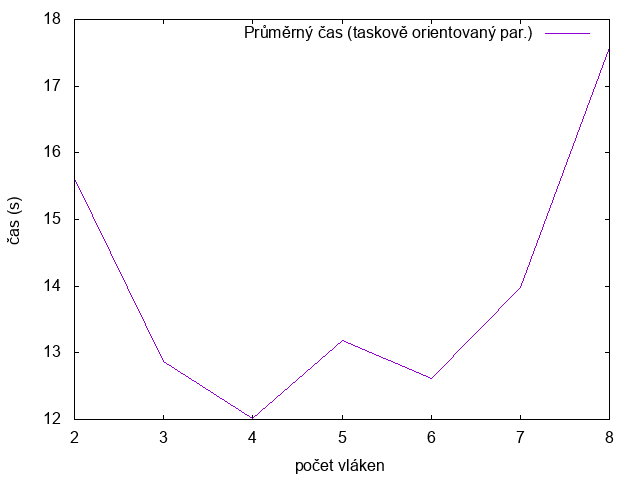
\includegraphics[width=0.8\textwidth]{assets/parallel-task-oriented.png}
    \caption{Taskový paralelismus -- závislost na počtu vláken}
    \label{fig:task}
\end{figure}

\subsection{Datově orientovaný paralelismus}

Pro taskově orientovaný paralelismus jsem zvolil stejný vstupní soubor a měření provedl na stejném vzorku vláken.
Protože výpočet opět probíhá paralelně, měření by mělo mít podobný výsledek jako u taskového paralelismu.
Výsledné časy mohou být zatížené tím, že jednotlivá vlákna vždy pracují s velkými instancemi, což by časovou náročnost mohlo negativně ovlivnit.

Graf \ref{fig:data} znázorňuje časovou náročnost tohoto řešení.
Proti všem očekáváním je výsledek podstatně horší, než u datového paralelismu.
Časy ovšem přesahují i složitost sekvenčního řešení.

Pro ověření správnosti měření jsem proto sledoval zatížení jednotlivých vláken v průběhu výpočtu.
Pro malý počet vláken program dlouho pracuje sekvenčně, to je zapříčeněno sestavováním fronty na začátku výpočtu.
Po sestavení fronty se vláknům předávájí počáteční stavy, které jsou ale příliš velké a nevytěžují vlákna rovnoměrně.

\begin{figure}[H]
    \centering
    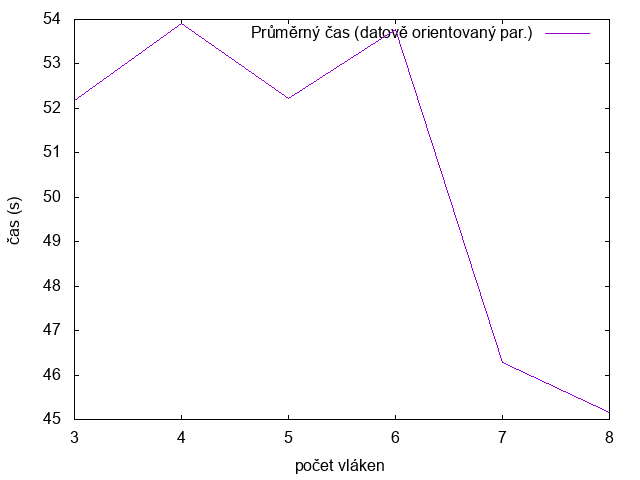
\includegraphics[width=0.8\textwidth]{assets/parallel-data-oriented.png}
    \caption{Datově paralelismus -- závislost na počtu vláken (velikost vstupní fronty 8)}
    \label{fig:data}
\end{figure}

Abych svou domněnku o závislosti výpočtu na počtu vláken potvrdil rozhodl jsem se měření opakovat s různými velikostmi počáteční fronty.
Při měření jsme vyzkoušel fronty o velikost 20, 30 40 a 50.
Přestože u velikosti 50 čas mírně poklesl, nebyl rozdíl větší než $10\%$.

Poslední měření jsem provedl na frontě o velikosti 70 aby zjistil, jestli nenastane klesající trend.
Pro tuto velikost už měření dosáhlo velmi dobrých výsledků.
Zlepšení u běhu na 8 vláknech dosáhlo vynikajících $90\%$ (tedy čas klesl na $10\%$ původního měření).
Výsledek měření je vidět na obrázku \ref{fig:data-2}

\begin{figure}[H]
    \centering
    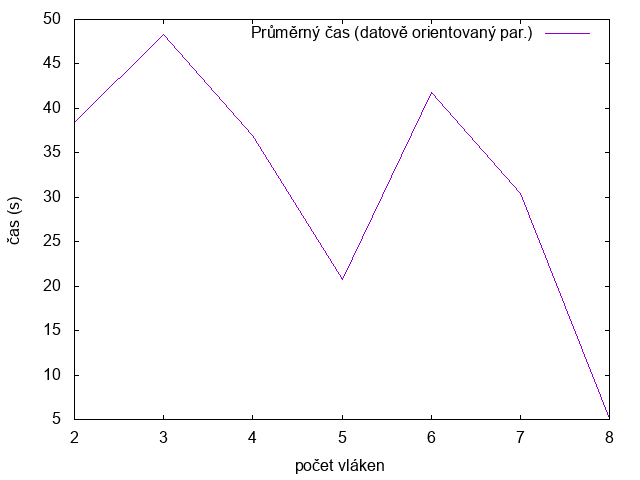
\includegraphics[width=0.8\textwidth]{assets/parallel-data-oriented-2.png}
    \caption{Datově paralelismus -- závislost na počtu vláken (velikost vstupní fronty 70)}
    \label{fig:data-2}
\end{figure}

Při efektivitě pro 8 souběžných vláken odpovídá doba výpočtu přibližně poměru $\frac{t}{n}$, který jsem od měření očekával.
Algoritmus s tímto nastavením je efektivnějíší než taskový paralelismus.

\subseciton{Paralelismus s MPI}

Jak jsem zmínil v úvodu kapitoly o měření, testovací data pro paralelní výpočet v klastru se mi nepodařilo získat.
Měřit efektivitu na osobním zařízení nemá vypovídací hodnotu, protože na jednom počítači degraduje na datový paralelismus, který je ale navíc zatížen meziprocesovou komunikací.
Z tohoto důvodu jsem měření \textit{MPI} vynechal.

\section{Závěr}

\end{document}